\chapter{Проектируем конкурентное приложение}
\begin{wrapfigure}{r}{0.35\linewidth}
    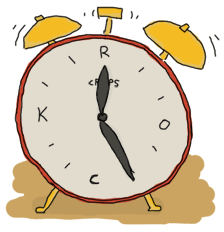
\includegraphics[width=1\linewidth]{clock.png}
\end{wrapfigure}
Всё это, конечно, здорово.
Вы получили представление о концепциях, но, опять же, мы с самого начала книги занимались лишь игрушечными примерами: калькуляторами, деревьями, ездили из Хитроу в Лондон и т.д.
Пора сделать что\--нибудь более интересное с точки зрения обучения.
Мы напишем небольшое приложение на конкурентном Erlang.
Приложение будет простым и взаимодействие с ним будет осуществляться посредством строковых команд.
Кроме того, оно будет приносить пользу и его функциональность можно будет наращивать.

Я немного неорганизованный человек.
Я теряюсь в домашних заданиях, благоустройстве квартиры, этой книге, работе, совещаниях, встречах и прочем.
У меня есть дюжина списков с задачами, которые я забываю сделать, или просто не нахожу для них времени.
Надеюсь, вам тоже иногда нужно напоминать о делах (хоть ваш разум  и не блуждает так же часто как мой).
Мы напишем приложение, которое уведомляет вас о необходимости что\--либо сделать и напоминает о встречах.
\section{Разбираем задачу}
Перво\--наперво нужно понять, что мы вообще собираемся сделать.
Вы скажете: <<Напоминалку>>.
<<Ну, конечно>>, \--- скажу я.
Но это ещё не всё.
Как мы собираемся взаимодействовать с программой?
Что она должна для нас делать?
Как представить программу при помощи процессов?
Как узнать, какие нужно отсылать сообщения?

Как говорится: "Ходить по воде и разрабатывать программное обеспечение по техническому заданию одинаково просто, если и то и другое заморожено."
Так что давайте разработаем технические условия и будем их придерживаться.
Наша программа позволит совершать следующие действия:
\begin{itemize}
\item Добавлять событие.
У событий может быть крайний срок исполнения (момент времени, о котором необходимо предупредить), наименование события и его описание.
\item Показывать предупреждение, когда подошло время.
\item Отменять событие по его имени.
\item Не хранить данные на диске.
    Для демонстрации архитектурных концепций, которые мы рассмотрим, хранение совершенно излишне.
Для настоящего приложения это, конечно никуда не годится, но я покажу, куда можно вставить код, если вам захочется реализовать эту функциональность, и укажу на несколько полезных функций, которые могли бы вам в этом помочь.
\item Так как постоянного хранилища у нас нет, нам нужно иметь возможность изменять код во время исполнения.
\item Общение с программой будет осуществляться через командную строку, но мы должны предусмотреть возможность последующего расширения  средств взаимодействия (добавить, скажем, графический интерфейс, доступ через веб\--страницу, через систему обмена мгновенными сообщениями (instant messaging), е\--мейл и прочее).
\end{itemize}

Для нашей программы я избрал такой способ организации:
\begin{figure}[h!]
    \centering
    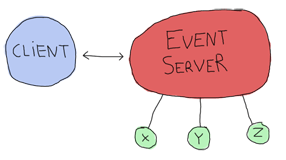
\includegraphics[width=0.4\textwidth]{reminder-structure.png}
\end{figure}

Где клиент, сервер событий и x, y, z представлены в виде процессов.
Вот что каждый из них может делать:
\subsection{Сервер событий}
\begin{itemize}
\item Принимает подписки от клиентов
\item Передаёт уведомления от процессов, генерирующих события, каждому подписчику
\item Принимает сообщения о добавлении событий (и необходимости запуска процессов x, y, z)
\item Может принимать сообщения об отмене события, и последующем убийстве процессов\--генераторов событий
\item Может быть остановлен клиентом
\item Его код может быть перезагружен из оболочки.
\end{itemize}
\subsection{Клиент}
\begin{itemize}
\item Подписывается на события у сервера событий и получает уведомления посредством сообщений.
Используя этот механизм, можно легко спроектировать группу клиентов, которые создают подписку на сервере событий.
Каждый клиент потенциально может служить шлюзом к различным точкам взаимодействия, упомянутым выше (графический интерфейс, веб\--страница, программа обмена мгновенными сообщениями, е\--мейл и т.д.)
\item Запрашивает у сервера создание события с необходимыми параметрами
\item Совершает к серверу запрос на отмену события
\item Отслеживает сервер (на случай если тот прекратит работу)
\item При необходимости останавливает сервер событий
\end{itemize}
\subsection{x, y и z}
\begin{itemize}
\item С их помощью обозначаются уведомления, готовые к запуску (они реализованы в виде таймеров, связанных с сервером событий)
\item Отсылают сообщение серверу событий по истечении заданного периода
\item Получают сообщение об отмене и умирают
\end{itemize}

Обратите внимание, что все клиенты (IM, почта и т.д., которые в этой книге не реализованы) получают уведомления обо всех событиях, а отмена не входит в список вещей, о которых следует предупреждать клиентов.
Эта программа написана для нас с вами, поэтому предполагается, что её будет запускать только один пользователь.

Вот более сложная схема, с указанием всех возможных сообщений:
\begin{figure}[h!]
    \centering
    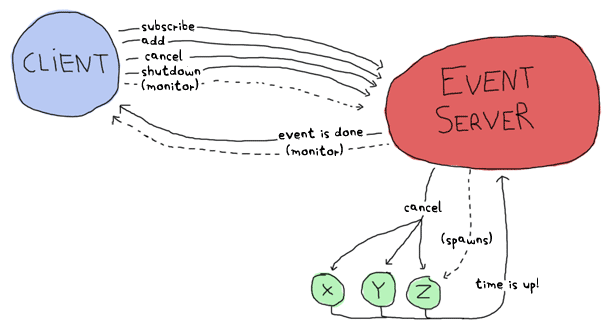
\includegraphics[width=0.7\textwidth]{reminder-bubbles-and-arrows.png}
\end{figure}

Здесь указан каждый процесс, который мы будем использовать.
Стрелки обозначают передаваемые сообщения.
С их помощью мы записали высокоуровневый протокол взаимодействия, ну или хотя бы его основу.

Нужно заметить, что для уведомлений мы используем по процессу на каждое событие.
Это слишком расточительно, и такое решение будет плохо масштабироваться в реальной задаче.
Но для приложения, единственным пользователем которого будете только вы, это вполне уместно.
Можно было бы решить эту проблему иначе, и использовать, к примеру, функцию \href{http://erldocs.com/R15B/stdlib/timer.html\#send_after/2}{timer:send\_after/2-3}, позволив тем самым избежать порождения большого количества процессов.
\clearpage
\section{Определяем протокол}
\label{defining-the-protocol}
Теперь, когда мы знаем что должен передавать каждый компонент и каковы его функции, неплохо было бы составить список всех передаваемых сообщений, и установить их вид.
Начнём с взаимодействия между клиентом и сервером событий:
\begin{figure}[h!]
    \centering
    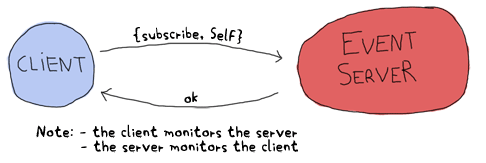
\includegraphics[width=0.6\textwidth]{reminder-subscribe.png}
\end{figure}

Я решил использовать два монитора, так как между клиентом и сервером нет явной зависимости.
Конечно, клиент без сервера работать не сможет, но сервер без клиента будет существовать без проблем.
Здесь можно было бы использовать связь (link), но мы хотим, чтобы функциональность нашей системы могла расширяться за счёт различных клиентов, поэтому мы не можем просто предположить, что после остановки сервера любой клиент тоже захочет аварийно завершиться.
Мы также не можем рассчитывать на то, что клиент можно превратить в системный процесс, и он начнёт улавливать завершения (exits) в случае смерти сервера.
Перейдём к следующему набору сообщений:
\begin{figure}[h!]
    \centering
    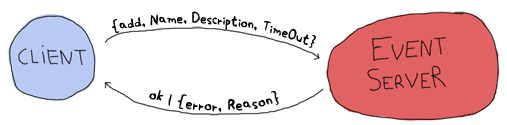
\includegraphics[width=0.6\textwidth]{reminder-add.png}
\end{figure}

Здесь мы добавляем на сервере событий ещё одно событие.
Клиенту высылается подтверждение в виде атома \ops{ok}, за исключением случаев, когда что\--то пошло не так (например, TimeOut был передан в неверном формате.)
Обратная операция удаления событий может быть совершена следующим образом:
\begin{figure}[h!]
    \centering
    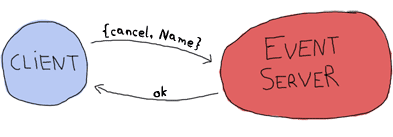
\includegraphics[width=0.6\textwidth]{reminder-remove.png}
\end{figure}

Позже сервер событий может отослать уведомление о том, что событие наступило:
\begin{figure}[h!]
    \centering
    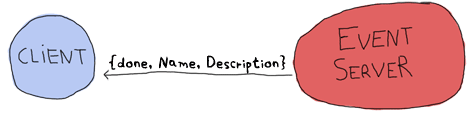
\includegraphics[width=0.6\textwidth]{reminder-cs-done.png}
\end{figure}

Нам осталось определить пару особых случаев: когда необходимо остановить сервер, и когда сервер аварийно завершается:
\begin{figure}[h!]
    \centering
    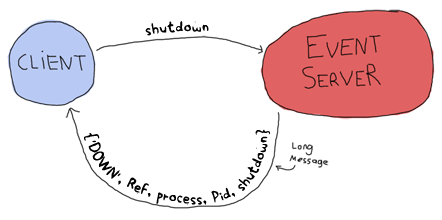
\includegraphics[width=0.6\textwidth]{reminder-shutdown.png}
\end{figure}

Прямое подтверждение об остановке  сервера не отсылается, так как о случившемся нас предупредит монитор.
Вот, в общем\--то и всё, что будет происходить между клиентом и сервером событий.
Перейдём к сообщениям, передаваемым между сервером событий и самими процессами событий.

Перед тем как мы приступим к их описанию, я бы хотел заметить, что неплохо было бы установить связи (links)  между сервером событий и событиями.
Сделать это нужно по той причине, что если сервер умирает, нам нужно чтобы все события умерли вместе с ним \--- без сервера в их существовании нет никакого смысла.

Хорошо, вернёмся к событиям.
Когда сервер событий их создаёт, он присваивает каждому особый идентификатор (имя события).
Как только приходит время какого\--нибудь события, сервер должен отослать об этом уведомление:
\begin{figure}[h!]
    \centering
    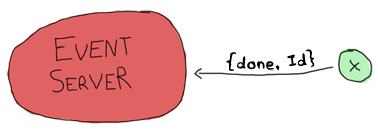
\includegraphics[width=0.6\textwidth]{reminder-es-done.png}
\end{figure}

\clearpage
Событие, в свою очередь, должно ожидать от сервера событий сигналы об отмене:
\begin{figure}[h!]
    \centering
    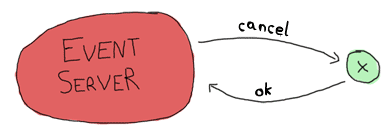
\includegraphics[width=0.6\textwidth]{reminder-cancel.png}
\end{figure}

Мы почти закончили.
Нам потребуется ещё одно последнее сообщение, которое позволит обновлять код сервера:
\begin{figure}[h!]
    \centering
    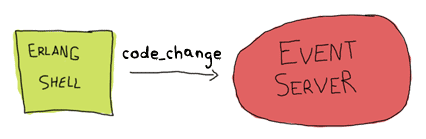
\includegraphics[width=0.6\textwidth]{reminder-code-change.png}
\end{figure}

Отвечать на это сообщение нет необходимости.
Когда мы реализуем эту часть нашей программы, вы поймёте почему мы можем так делать.

Теперь у нас есть и протокол общения, и приблизительная структура иерархии процессов.
Можно наконец\--то приступить к воплощению нашего проекта в жизнь.
\section{Заложим\--ка основы}
\begin{wrapfigure}{r}{0.4\linewidth}
    
\includegraphics[width=1\linewidth]{cement.png}
\end{wrapfigure}
Для начала мы должны создать стандартный набор директорий, принятый в Erlang.
Вот как он выглядит:

ebin/

include/

priv/

src/

В директорию \ops{ebin/} попадают скомпилированные файлы.
Директория \ops{include/} используется для хранения файлов \ops{.hrl}, предназначенных для включения другими приложениями; файлы с расширением \ops{.hrl}, доступные лишь текущему приложению (private), обычно хранятся в директории \ops{src/}.
Директория \ops{priv/} содержит исполняемые файлы, которые могут взаимодействовать с Erlang.
К их числу относятся некоторые драйверы и прочее в этом духе.
В нашем проекте мы эту директорию использовать не будем.
Ну и последняя директория \--- \ops{src/}, в ней находятся все файлы \ops{.erl}.

Описанная структура директорий может немного варьироваться в стандартных проектах Erlang.
Для хранения некоторых конфигурационных файлов может добавляться директория \ops{conf/}, для документации \ops{doc/} и \ops{lib/} \--- для сторонних библиотек, которые ваше приложение использует во время исполнения.
Зачастую различные Erlang\--продукты, представленные на рынке, используют имена отличные от указанных, но четыре имени, упомянутые выше, обычно не меняются, так как они являются частью \href{http://www.erlang.org/doc/design_principles/applications.html\#id71171}{стандартных приёмов (standard practices) OTP}.
\section{Модуль для работы с событиями}
\label{an-event-module}
Зайдите в директорию \ops{src/} и откройте модуль \href{file:///home/max/prog/learnyousomeerlang/original/learnyousomeerlang.com/static/erlang/event.erl}{event.erl}, который реализует события x, y и z, отмеченные на приведённых ранее рисунках.
Я начинаю именно с этого модуля, так как у него меньше всего зависимостей.
Мы сможем попытаться его запустить, не реализуя сервер событий или функции клиента.

Перед тем как мы начнём писать код, я должен упомянуть, что разработанный нами протокол неполон.
Он помогает представить те данные, которые будут пересылаться между процессами, но не описывает подробности пересылки.
Как работает адресация? 
Что мы при этом используем \--- ссылки или имена и т.д.
Большинство сообщений будут завёрнуты в кортеж вида \ops{\{Pid, Ref, Message\}}, где \emph{Pid} \--- отправитель и \emph{Ref} \--- уникальный идентификатор сообщения, который помогает определить, от кого был получен ответ.
Если бы перед ожиданием ответов мы отослали множество сообщений, то без ссылок нам не удалось бы понять, какому сообщению соответствует каждый из ответов.

Начинаем.
Ядром процессов, исполняющих код модуля \ops{event.erl} будет функция \ops{loop/1}, основа которой будет выглядеть приблизительно следующим образом, если вы помните протокол:
\begin{lstlisting}[style=erlang]
loop(State) ->
    receive
        {Server, Ref, cancel} ->
            ...
    after Delay ->
        ...
    end.
\end{lstlisting}

Здесь показан поддерживаемый нами тай\--маут, который оповещает о наступлении события, а также способ отмены события сервером.
В цикле вы можете заметить переменную \emph{State}.
Эта переменная будет содержать значение тайм\--аута (в секундах) и имя события (необходимое для отсылки сообщения \ops{\{done, Id\}}.)
Для отсылки уведомлений серверу событий также понадобится его pid.

Вся эта информация вполне годится для размещения в состоянии, хранимом в цикле.
Для этого объявим в начале файла запись \ops{state}:
\begin{lstlisting}[style=erlang]
-module(event).
-compile(export_all).
-record(state, {server,
                name="",
                to_go=0}).
\end{lstlisting}

Состояние объявлено, теперь можно немного усовершенствовать цикл:
\begin{lstlisting}[style=erlang]
loop(S = #state{server=Server}) ->
    receive
        {Server, Ref, cancel} ->
            Server ! {Ref, ok}
    after S#state.to_go*1000 ->
        Server ! {done, S#state.name}
    end.
\end{lstlisting}

Умножение на тысячу используется для перевода значения \ops{to\_go} из секунд в миллисекунды.\\
\colorbox{lorange}
{
\begin{minipage}{1.0\linewidth}
    \textbf{Не забывайтесь:}\\
    Сейчас я расскажу об изъяне языка!
    Я связываю переменную <<Server>> в заголовке функции, так как она используется при сопоставлении с образцом в секции receive.
    Помните, что \ref{records} ~записи \--- это хак!
    \ops{S\#state.server} тайком разворачивается в выражение \ops{element(2, S)}, которое не является шаблоном, пригодным для сопоставления.

    Для выражения \ops{S\#state.to\_go}, следующего за \ops{after}, этот механизм срабатывает нормально, так как его обработку можно отложить на более позднее время.
\end{minipage}
}

А теперь проверим цикл:
\begin{lstlisting}[style=erlang]
6> c(event).
{ok,event}
7> rr(event, state).
[state]
8> spawn(event, loop, [#state{server=self(), name="test", to_go=5}]).
<0.60.0>
9> flush().
ok
10> flush().
Shell got {done,"test"}
ok
11> Pid = spawn(event, loop, [#state{server=self(), name="test", to_go=500}]).
<0.64.0>
12> ReplyRef = make_ref().
#Ref<0.0.0.210>
13> Pid ! {self(), ReplyRef, cancel}.
{<0.50.0>,#Ref<0.0.0.210>,cancel}
14> flush().
Shell got {#Ref<0.0.0.210>,ok}
ok
\end{lstlisting}

Довольно насыщенный пример.
Сначала мы импортируем запись (record) из модуля обработки событий командой \ops{rr(Mod)}.
Затем запускаем цикл обработки событий, для которого сервером выступает оболочка (\ops{self()}).
Заданное событие должно произойти через 5 секунд.
Выражение в 9\--ой строке было запущено через 3 секунды, а в 10\--ой \--- через 6 секунд.
Как видите, со второй попытки мы получили сообщение \ops{\{done, "test"\}}.

Затем я пытаюсь воспользоваться командой отмены (для ввода которой c запасом выделяется 500 секунд).
Видно, как я создаю ссылку, посылаю сообщение и получаю ответ, используя ту же самую ссылку.
Я могу быть уверен, что полученное сообщение \ops{ok} пришло именно от заявленного процесса, а не какого\--либо другого существующего в системе.

Сообщение отмены завёрнуто в ссылку, а сообщение \ops{done} \--- нет.
Так сделано просто потому, что мы не ожидаем получить \ops{done} от какого\--либо определённого процесса (сгодится любой, мы не будем проводить сопоставление в receive), и отвечать на это сообщение мы тоже не намерены.
Я бы хотел проделать заранее ещё один тест.
Что будет, если событие произойдёт в следующем году?
\begin{lstlisting}[style=erlang]
15> spawn(event, loop, [#state{server=self(), name="test", to_go=365*24*60*60}]).
<0.69.0>
16>
=ERROR REPORT==== DD-MM-YYYY::HH:mm:SS ===
Error in process <0.69.0> with exit value: {timeout_value,[{event,loop,1}]}
\end{lstlisting}

Ой.
Кажется мы наткнулись на ограничение реализации.
Оказывается на значение тайм\--аута в Erlang накладывается ограничение в 50 дней (в миллисекундах).
Может быть, эта особенность и не столь важна, но я продемонстрировал эту ошибку по трём причинам:
\begin{enumerate}
    \item Я напоролся на этот нюанс, когда глава была наполовину написана, и я разрабатывал и тестировал для неё модуль.
    \item Конечно же, Erlang не с любой задачей справляется идеально, а здесь мы сталкиваемся с последствиями работы с таймерами, не предусмотренным разработчиками способом.
    \item Но вообще\--то это не проблема; давайте её обойдём.
\end{enumerate}

Для исправления этого недостатка я решил написать функцию, которая разделяла бы значение слишком длинного тайм\--аута на несколько частей.
От функции \ops{loop/1} это тоже потребует некоторого содействия.
Короче говоря, мы просто разделим время на равные части по 49 дней (так как ограничение равно приблизительно 50 дням), а затем к этим равным частям добавим остаток.
Полная сумма значений в этом списке должна быть равна исходному временному промежутку:
\begin{lstlisting}[style=erlang]
%% Because Erlang is limited to about 49 days (49*24*60*60*1000) in
%% milliseconds, the following function is used
normalize(N) ->
    Limit = 49*24*60*60,
    [N rem Limit | lists:duplicate(N div Limit, Limit)].
\end{lstlisting}

Функция \ops{\href{http://erldocs.com/R15B/stdlib/lists.html\#duplicate/2}{lists:duplicate/2}} принимает вторым аргументом данное выражение и повторяет его столько раз, сколько определено значением первого аргумента (\ops{[a,a,a] = lists:duplicate(3, a)}).
Если бы мы передали функции \ops{normalize/1} значение \ops{98*24*60*60+4}, то она бы возвратила \ops{[4,4233600,423360]}.
Для работы с новым форматом функция \ops{loop/2} принимает следующий вид:
\begin{lstlisting}[style=erlang]
%% Loop uses a list for times in order to go around the ~49 days limit
%% on timeouts.
loop(S = #state{server=Server, to_go=[T|Next]}) ->
    receive
        {Server, Ref, cancel} ->
            Server ! {Ref, ok}
    after T*1000 ->
        if Next =:= [] ->
            Server ! {done, S#state.name};
            Next =/= [] ->
            loop(S#state{to_go=Next})
        end
    end.
\end{lstlisting}

Можете попробовать её запустить, она будет работать как и прежде, но ко всему прочему сможет обрабатывать тайм\--ауты длиной в несколько лет.
Работает этот механизм следующим образом: функция извлекает из списка \ops{to\_go} первый элемент и переходит в состояние ожидания на период, равный значению этого элемента.
Когда ожидание окончено, проверяется, есть ли в списке следующий элемент.
Если список пуст, то тайм\--аут окончен, и сервер получает об этом уведомление.
В противном случае процесс повторяется для всех остальных элементов списка, до полного их исчерпания.
